\section{Avaliação}\label{sec:avaliacao}
\begin{frame}{Avaliação}
	\begin{itemize}
		\setlength{\itemsep}{1em}
		\item<1-> Termo de Consentimento Livre e Esclarecido
		\item<1-> Tarefas:
		\begin{itemize}
			\setlength{\itemsep}{0.5em}
			\item<1-> 9 tarefas
		\end{itemize}
		\item<1-> Questionário:
		\begin{itemize}
			\setlength{\itemsep}{0.5em}
			\item<1-> Baseado nas heurísticas de Nielsen
			\item<1-> 48 questões
		\end{itemize}
	\end{itemize}	
\end{frame}

\subsection{Resultados}
\begin{frame}{Resultados}
	\begin{itemize}
		\setlength{\itemsep}{1em}
		\item<1-> 7 participantes, sendo 1 com deficiência visual	
		\item<1-> Fluxo da aplicação condizente com a expectativa dos usuários 
		\item<1-> \textit{Consistência e Padronização}, \textit{Prevenção de Erros} e \textit{Projeto Estético e Minimalista} foram os critérios melhor avaliados
		\item<1-> Os itens referentes a \textit{Reconhecimento ao Invés de Memorização} apresentaram baixa aprovação por parte dos avaliadores
	\end{itemize}
\end{frame}

\begin{frame}{Tempo Médio de Execução das Tarefas}
	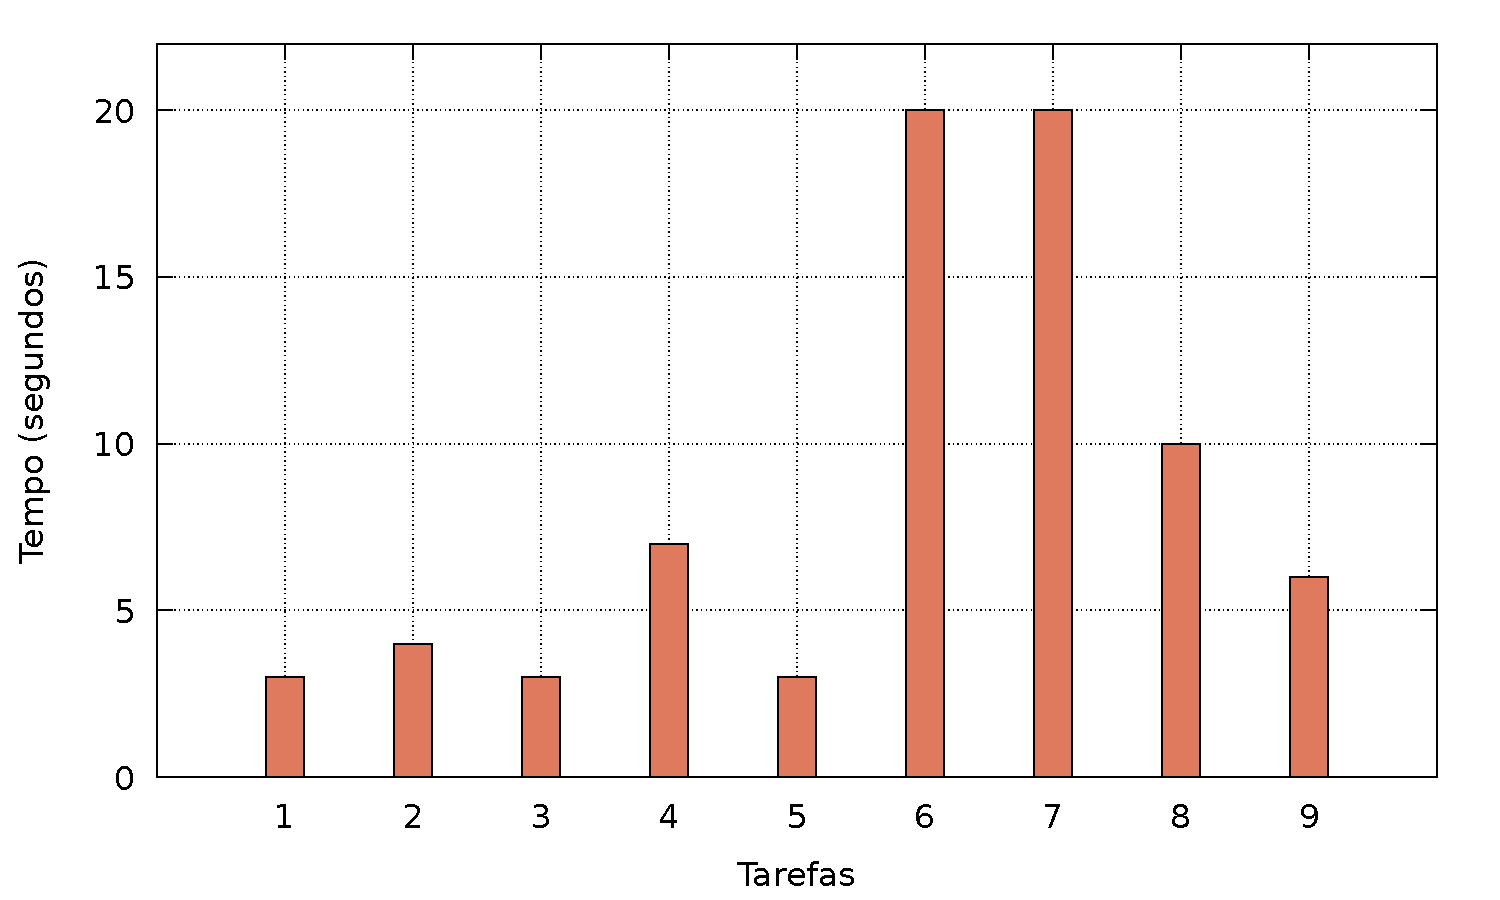
\includegraphics[width=1\linewidth]{../charts/tempo-sem-dv.pdf}<1-1>
	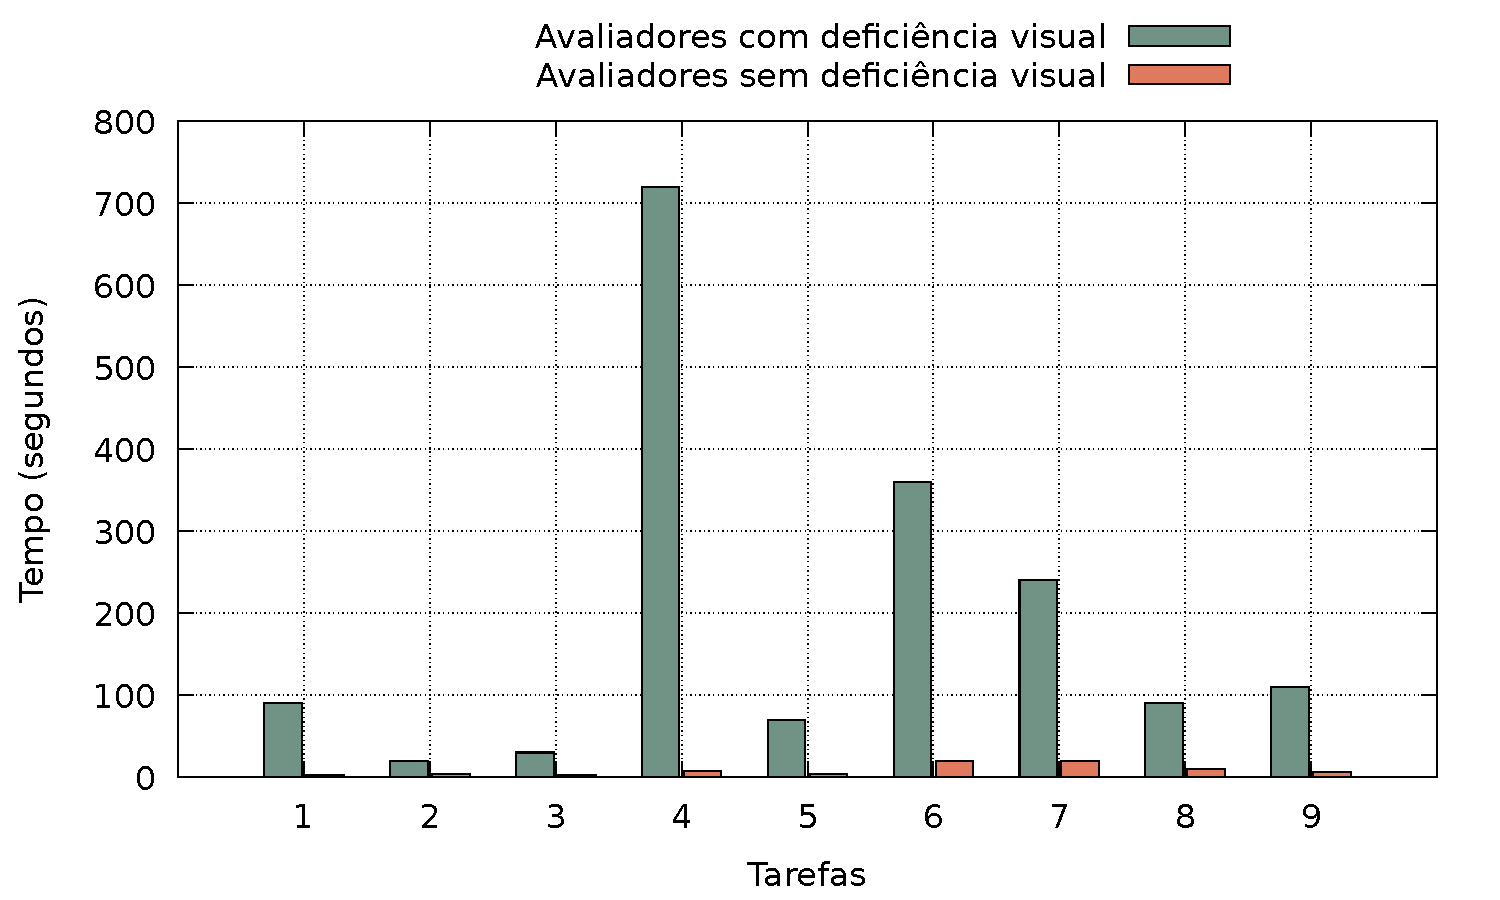
\includegraphics[width=1\linewidth]{../charts/tempo.pdf}<2-2>
\end{frame}

\begin{frame}{Reconhecimento, Diagnóstico e Recuperação de Erros}
	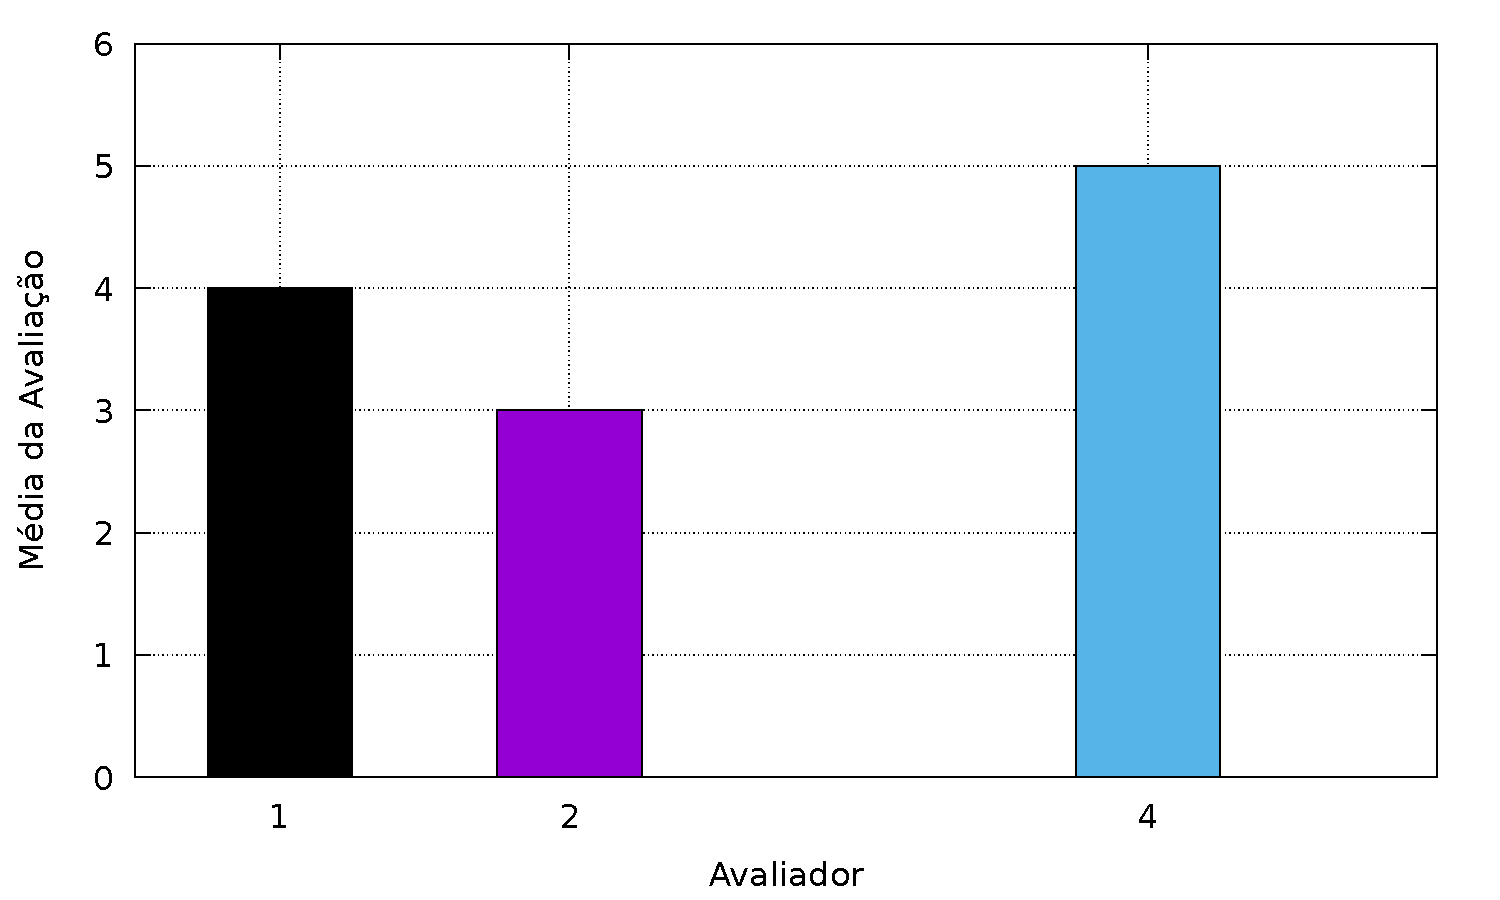
\includegraphics[width=1\linewidth]{../charts/qt9.pdf}<1-1>
\end{frame}

\begin{frame}{Sugestões e Melhorias}
	\begin{itemize}
		\setlength{\itemsep}{1em}
		\item<1-> Sugestão de restaurantes na barra de busca
		\item<1-> Tela de Favoritos \textbf{não ser} a tela inicial da aplicação
		\item<1-> Botão de Página Inicial
		\item<1-> \emph{Feedback} após a inserção de filtros
		\item<1-> Sistema de busca dentro do cardápio
		\item<1-> Categorias mais intuitivas
		\item<1-> Menos categorias
	\end{itemize}
\end{frame}
